\subsection{Backgrounds: Hadronic channel}
\label{subsec:bkg_hadronic}

The main backgrounds in this channel are semileptonic $\ttbar$, $\Wjets$, and $\Z(\Nu\Nu)+$jets, and control regions enriched in these backgrounds are defined in the following. Also, a control region for QCD is defined to validate that the background is expected to be small.

\subsubsection{Control region for \texorpdfstring{$\ttbar$}{ttbar}}
\label{subsubsec:bkg_hadronic_ttbar}

A control region enriched in semileptonic $\ttbar$ can be obtained by requiring exactly one ``Tight'' electron or muon with $M_T<160\:\GeV$, while keeping all other selection requirements.\iffalse For the categories with boosted top tags, the subjet $\Bot$-tag requirements are dropped.To obtain a $\met$ template, the four-momentum of the lepton is removed and it is this lepton subtracted $\met$ quantity that must be greater than $250\:\GeV$.\fi From the studies shown in Appendix ~\ref{app:CR}, we determine that removal of the lepton four-momentum from the $\met$ in this control region isn't necessary in order to model the $\met$ distribution in the signal region. The yields are listed in Table~\ref{tab:hadronic_bkg_tt1l_yields}. The \iffalse lepton subtracted \fi $\met$ distributions in the control region for the inclusive selection is shown in Fig.~\ref{fig:incl_hadronic_1l_fmet} for both the electron and muon selection. 

\begin{table}[!ht]
\centering
\begin{tabular}{|c|r|r|}
\hline
  Process & \multicolumn{1}{|c|}{Electron Channel} & \multicolumn{1}{|c|}{Muon Channel} \\
\hline
  Diboson         & $   1.09 \pm  0.33$ & $  0.97 \pm  0.27$ \\
  \Zjets            & $ 0.58 \pm  0.22$ &$4.07 \pm  1.23$ \\
  Single \Top    & $ 52.12 \pm 1.48$ &  $57.99 \pm  1.51$ \\
  \Wjets            & $   34.97 \pm  1.10$ & $  46.53 \pm  1.53$ \\
  $\ttbar$   & $   618.07 \pm  3.17$ & $  710.05 \pm  3.30$ \\
  QCD        & $ 0.00 \pm 0.00$ & $0.00\pm  0.00$ \\
\hline
SM expected     & $706.83 \pm 3.69$ & $819.61 \pm 4.14$ \\
 \hline
  Observed        & $719.00 \pm 0.00$ & $883.00 \pm 0.00$ \\
\hline
  $M_\chi=1\:\GeV\:, M_\phi=10\:\GeV\:$       & $  1.30 \pm  0.12$ &  $2.30  \pm  0.16$ \\
\hline
\end{tabular}
\caption{Expected and observed yields for $1.3\:\ifb$ in the $\ttbar$ control region for the hadronic channel.}
\label{tab:hadronic_bkg_tt1l_yields}
\end{table}

\begin{figure}[htbp]
  \centering
  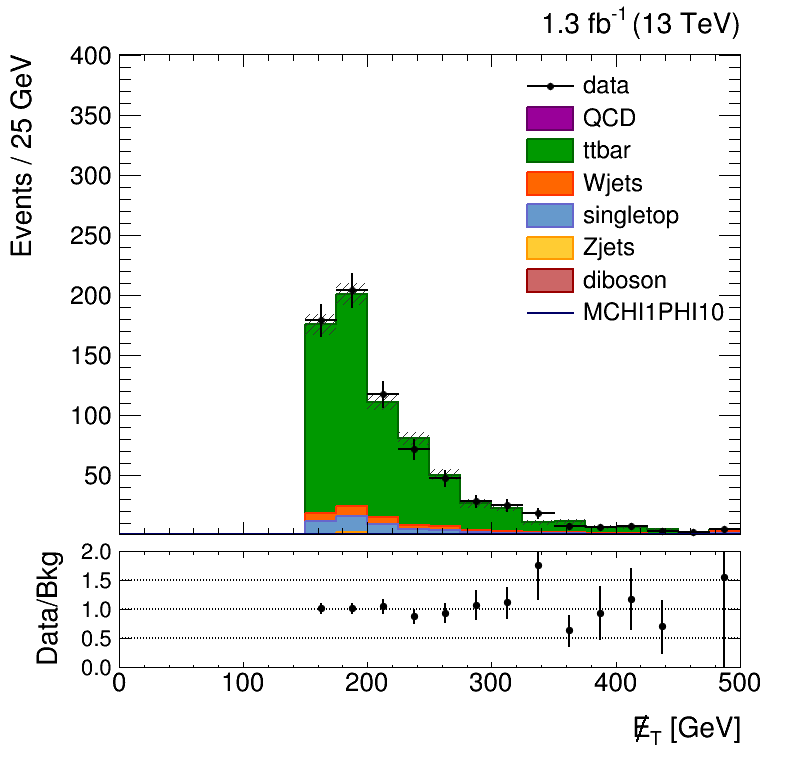
\includegraphics[width=0.48\textwidth]{figures/hMETlinear_CRttbar_el.png}
  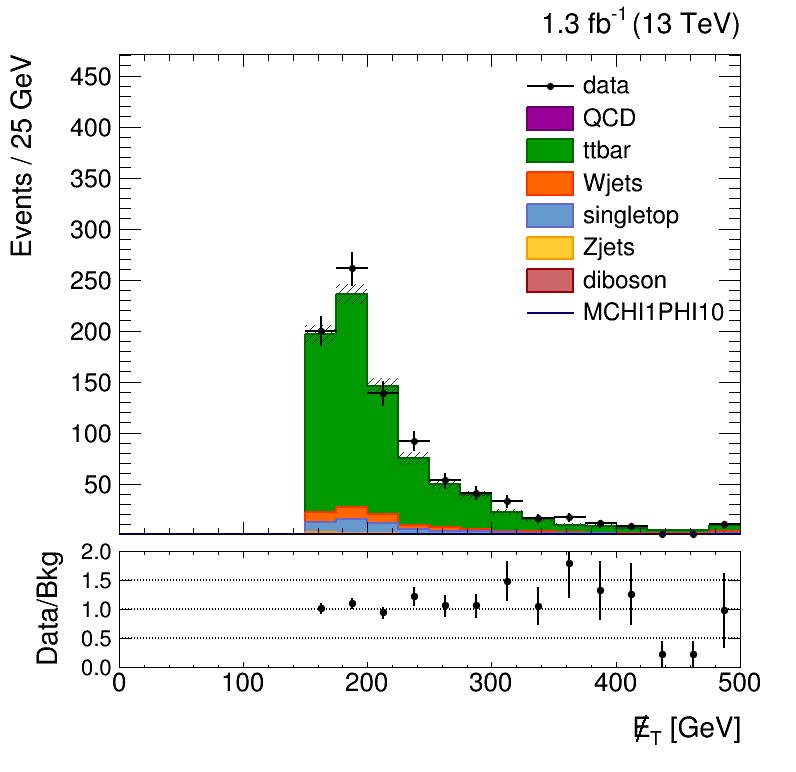
\includegraphics[width=0.48\textwidth]{figures/hMETlinear_CRttbar_mu.png}
    \caption{The $\met$ distribution in the $\ttbar$ control region with electron (left) and muon (right) selection for the hadronic channel.}
  \label{fig:incl_hadronic_1l_fmet}
\end{figure}

\clearpage
\subsubsection{Control region for \texorpdfstring{$V+$jets}{Vjets}}
\label{subsubsec:bkg_hadronic_vjets}

By requiring no $\Bot$-tagged jets in the event and keeping all other cuts the same, a sample enriched in $\Wjets$ and $\Z(\Nu\Nu)+$jets can be obtained. From the studies shown in Appendix ~\ref{app:CR}, we determine that removal of the lepton four-momentum from the $\met$ in the $V+$jets control region isn't necessary in order to model the $\met$ distribution in the signal region. \iffalse For the categories with boosted top tags, the subjet $\Bot$-tag requirements are dropped.\fi  The yields are listed in Table~\ref{tab:hadronic_bkg_vjets_yields}. The $\met$ distributions in the control region for the inclusive selection is shown in Fig.~\ref{fig:incl_hadronic_0b_met}.

\begin{table}[!ht]
\centering
\begin{tabular}{|c|r|}
\hline
  Process & \\
\hline
  Diboson         & $ 33.10 \pm 1.89 $ \\
  \Zjets            & $681.22 \pm 3.91$ \\
  Single \Top    & $21.65 \pm 0.95 $ \\
  \Wjets            & $ 1341.57 \pm 11.81 $ \\
  $\ttbar$   & $    221.19 \pm 1.94$ \\
  QCD        & $ 19.54 \pm 2.96$ \\
\hline
SM expected     & $  2318.28 \pm 13.11$\\
 \hline
  Observed        & $2380.00 \pm 0.00$ \\
\hline
  $M_\chi=1\:\GeV\:, M_\phi=10\:\GeV\:$       & $ 2.76 \pm 0.18$ \\
\hline
\end{tabular}
\caption{Expected yields for $1.3\:\ifb$ in the $V+$jets control region for the hadronic channel.}
\label{tab:hadronic_bkg_vjets_yields}
\end{table}

\begin{figure}[htbp]
  \centering
  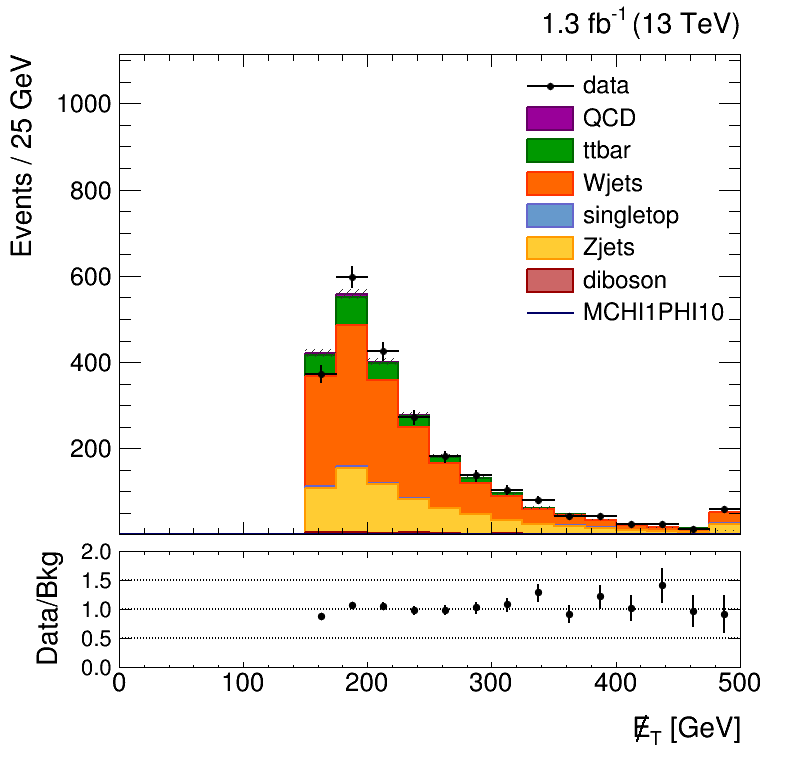
\includegraphics[width=0.48\textwidth]{figures/hMETlinear_CRvjets_0b.png}
  \caption{The $\met$ distribution in the $V+$jets control region for the hadronic channel.}
  \label{fig:incl_hadronic_0b_met}
\end{figure}

\subsubsection{Control region for \texorpdfstring{$\Wjets$}{Wjets}}
\label{subsubsec:bkg_hadronic_wjets}

A control region enriched in $\Wjets$ can be obtained by requiring a ``Tight'' electron or muon and no $\Bot$-tagged jets, while keeping all other selection requirements. \iffalse For the categories with boosted top tags, the subjet $\Bot$-tag requirements are dropped. \fi To obtain a $\met$ template, we do not remove the lepton four-momentum and require that this $\met$ quantity that must be greater than $250\:\GeV$. Studies that support retaining the lepton \pt\: are detailed in Appendix~\ref{app:CR}.The expected and observed yields are listed in Table~\ref{tab:hadronic_bkg_vjets_yields}. The \iffalse lepton subtracted \fi $\met$ distributions in the control region for the inclusive selection is shown in Fig.~\ref{fig:incl_hadronic_1l0b_fmet} for both the electron and muon selection.

\begin{table}[!ht]
\centering
\begin{tabular}{|c|r|r|}
\hline
  Process & \multicolumn{1}{|c|}{Electron Channel} & \multicolumn{1}{|c|}{Muon Channel} \\
\hline
  Diboson         & $  000000$ & $17.72 \pm 1.48$ \\
  \Zjets            & $20.61 \pm1.98$ &  $24.65 \pm 2.07$ \\
  Single \Top    & $ 23.65 \pm 0.98$ &  $30.23 \pm 1.13$ \\
  \Wjets            & $ 770.08 \pm 6.72$ & $  886.25 \pm 7.32$ \\
  $\ttbar$   & $   253.06 \pm 2.03$ & $  313.48 \pm 2.30$ \\
  QCD        & $ 3.13 \pm 1.32$ & $0.64 \pm 0.60$ \\
\hline
SM expected     & $1088.29 \pm 7.62$ & $1272.98 \pm 8.19$ \\
 \hline
  Observed        & $939.00 \pm 0.00$ & $1167.00 \pm 0.00$ \\
\hline
  $M_\chi=1\:\GeV\:, M_\phi=10\:\GeV\:$       & $  0.94 \pm  0.10$ &  $1.19  \pm  0.12$ \\
\hline
\end{tabular}
\caption{Expected and observed yields for $1.3\:\ifb$ in the $\Wjets$ control region for the hadronic channel.}
\label{tab:hadronic_bkg_wjets_yields}
\end{table}

\begin{figure}[htbp]
  \centering
  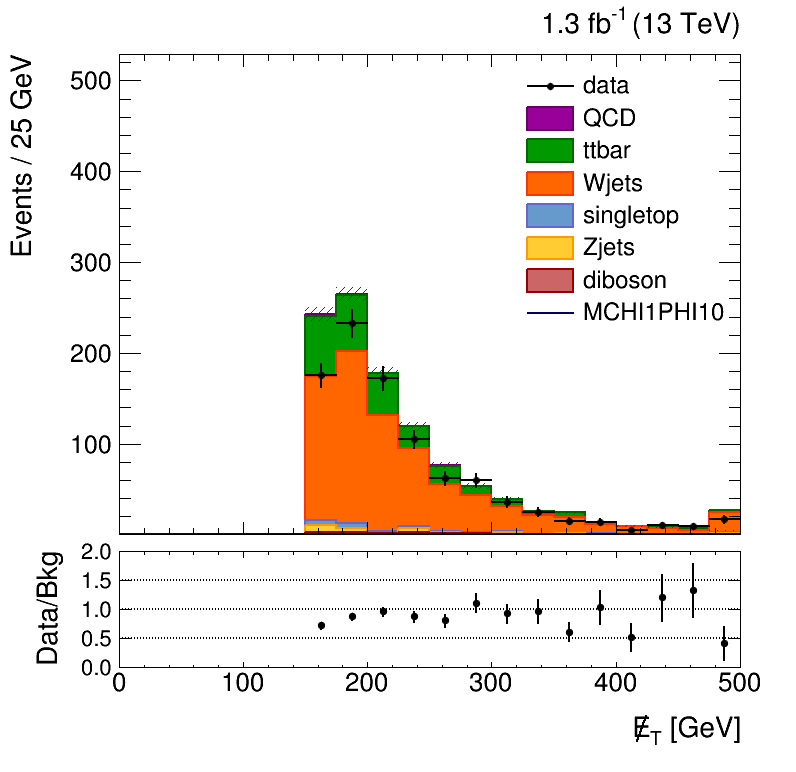
\includegraphics[width=0.48\textwidth]{figures/hMETlinear_CRwjets_el.png}
  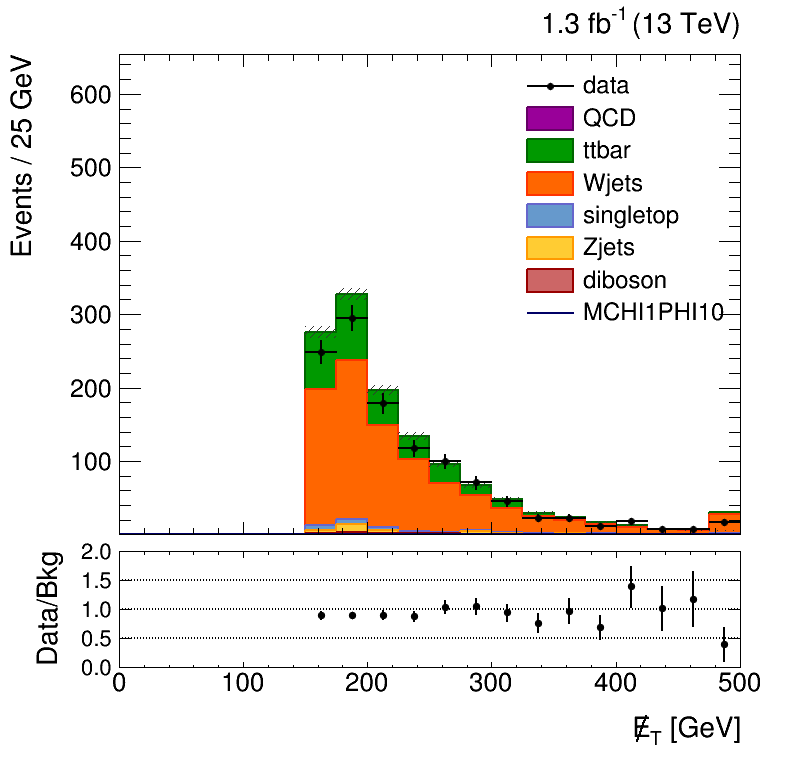
\includegraphics[width=0.48\textwidth]{figures/hMETlinear_CRwjets_mu.png}
  \caption{The $\met$ distribution in the $\Wjets$ control region for the hadronic channel for electron (left) and muon (right) selection.}
  \label{fig:incl_hadronic_1l0b_fmet}
\end{figure}


%2j/0b
%  *     Z+jets    954.88 +/-   6.92
%  *   single t    332.13 +/-   6.67
%  *     W+jets  42025.86 +/- 136.36
%  * t#bar{t}+V      0.75 +/-   0.10
%  * t#bar{t}(had)      0.16 +/-   0.16
%  * t#bar{t}(2l)    122.08 +/-   4.47
%  * t#bar{t}(1l)    639.34 +/-  10.22
%  ============
%     total bkg  44075.21 +/- 137.16
%      DM 1 GeV      3.41 +/-   0.37

%2j/2b
%  *     Z+jets      2.46 +/-   0.31
%  *   single t     31.57 +/-   2.11
%  *     W+jets     77.21 +/-   5.23
%  * t#bar{t}+V      0.11 +/-   0.04
%  * t#bar{t}(had)      0.00 +/-   0.00
%  * t#bar{t}(2l)     26.80 +/-   2.09
%  * t#bar{t}(1l)     71.75 +/-   3.42
%  ============
%     total bkg    209.91 +/-   6.93
%      DM 1 GeV      0.90 +/-   0.19


%2j/1b
%  *     Z+jets     78.01 +/-   1.91
%  *   single t    293.13 +/-   6.49
%  *     W+jets   3057.11 +/-  35.02
%  * t#bar{t}+V      1.07 +/-   0.12
%  * t#bar{t}(had)      0.00 +/-   0.00
%  * t#bar{t}(2l)    190.56 +/-   5.58
%  * t#bar{t}(1l)    700.46 +/-  10.70
%  ============
%     total bkg   4320.34 +/-  37.65
%      DM 1 GeV      6.13 +/-   0.50

\clearpage
\subsubsection{Control region for \texorpdfstring{$\Zjets$}{Zjets}}
\label{subsubsec:bkg_hadronic_zjets}

A control region enriched in $\Zjets$ can be obtained by requiring a pair of ``Tight'' electrons or muons, with dilepton mass between $60\:\GeV$ and $120\:\GeV$, and no $\Bot$-tagged jets, while keeping all other selection requirements. The agreement between the $\met$ distribution in the $\Zjets$ control and signal regions shown in Appendix~\ref{app:CR} validate the following extracted $\met$ distribution. \iffalse For the categories with boosted top tags, the subjet $\Bot$-tag requirements are dropped. \fi To obtain a $\met$ template for $\Z\To\Nu\Nu$, the four-momentum of the dilepton system is removed and it is the dilepton subtracted $\met$ that must be greater than $250\:\GeV$. The yields are listed in Table~\ref{tab:hadronic_bkg_zjets_yields}. The lepton subtracted $\met$ distributions in the control region for the inclusive selection is shown in Fig.~\ref{fig:incl_hadronic_2l0b_fmet}.

\begin{table}[!ht]
\centering
\begin{tabular}{|c|r|r|}
\hline
  Process & \multicolumn{1}{|c|}{$ee$} & \multicolumn{1}{|c|}{$\mu\mu$} \\
\hline
  Diboson         & $  3.70 \pm 0.47$ & $4.15 \pm 0.46$ \\
  \Zjets            & $134.70 \pm 4.50$ &  $213.82 \pm 5.85$ \\
  Single \Top    & $ 0.83 \pm 0.18$ &  $0.79 \pm 0.17$ \\
  \Wjets            & $ 0.35 \pm 0.12$ & $  0.21 \pm 0.11$ \\
  $\ttbar$   & $   10.52 \pm 0.41$ & $   16.72 \pm 0.53$ \\
  QCD        & $0.07 \pm 0.07$ & $ 1.63 \pm 1.08$ \\
\hline
SM expected     & $150.17 \pm 4.55$ & $237.33 \pm 5.99$ \\
 \hline
  Observed        & $170.00 \pm 0.00$ & $274.00 \pm 0.00$ \\
\hline
  $M_\chi=1\:\GeV\:, M_\phi=10\:\GeV\:$       & $  0.00 \pm 0.00$ &  $0.02 \pm 0.02$ \\
\hline
\end{tabular}

\caption{Expected yields for $1.3\:\ifb$ in the $\Zjets$ control region with dileptons for the hadronic channel.}
\label{tab:hadronic_bkg_zjets_yields}
\end{table}

\begin{figure}[htbp]
  \centering
  \includegraphics[width=0.48\textwidth]{figures/hMETNoLepLinear_CRzjets_el.png}
  \includegraphics[width=0.48\textwidth]{figures//hMETNoLepLinear_CRzjets_mu.png}
  \caption{The $\met$ distribution in the $\Zjets$ control region with dileptons for the hadronic channel with the double electron (left) and double muon (right) selection.}
  \label{fig:incl_hadronic_2l0b_fmet}
\end{figure}

%2j/0b
%  *     Z+jets   3240.14 +/-  12.37
%  *   single t      3.64 +/-   0.82
%  *     W+jets      0.15 +/-   0.09
%  *   t#bar{t}     14.71 +/-   1.55
%  * t#bar{t}+V      0.04 +/-   0.02
%  ============
%     total bkg   3258.69 +/-  12.49
%      DM 1 GeV      0.16 +/-   0.08

%2j/2b
%  *     Z+jets      8.49 +/-   0.58
%  *   single t      1.63 +/-   0.54
%  *     W+jets      0.00 +/-   0.00
%  *   t#bar{t}      0.82 +/-   0.37
%  * t#bar{t}+V      0.01 +/-   0.01
%  ============
%     total bkg     10.95 +/-   0.88
%      DM 1 GeV      0.04 +/-   0.04

%2j/1b
%  *     Z+jets    264.17 +/-   3.39
%  *   single t      6.72 +/-   1.11
%  *     W+jets      0.00 +/-   0.00
%  *   t#bar{t}     14.55 +/-   1.54
%  * t#bar{t}+V      0.13 +/-   0.04
%  ============
%     total bkg    285.56 +/-   3.88
%      DM 1 GeV      0.29 +/-   0.11

Another way to model the $\met$ distribution for $\Z(\Nu\Nu)+$jets is to use $\gamma+$jets events. The $\gamma+$jets yields are much higher than for $\Z(\Lep\Lep)+$jets, however theoretical corrections must be applied to the photon $\pt$ spectrum to make it more $\Z$-like, and this introduces some systematic uncertainty. The selection for the control region takes events passing the HLT\_Photon155 trigger, requires the leading photon in the event to have $\pt>100\:\GeV$, $|\eta|<2.5$ while excluding the barrel-endcap transition region ($1.4442<|\eta_{\mbox{\scriptsize{SC}}}|>1.556$), and to pass the ``Medium'' WP. All other signal region cuts are applied, including $\Bot$-tagging requirements. To obtain a $\met$ template for $\Z\To\Nu\Nu$, the four-momentum of the photon is removed and it is the photon subtracted $\met$ that must be greater than $200\:\GeV$. The yields are listed in Table~\ref{tab:hadronic_bkg_pho_yields}. The lepton subtracted $\met$ distributions in the control region for the inclusive selection is shown in Fig.~\ref{fig:incl_hadronic_pho_fmet}.

\begin{table}[!ht]
\centering
\begin{tabular}{|c|r|}
\hline
  Process & \\
\hline
  $\gamma+$jets  & $245.11 \pm 6.78$ \\
  QCD                   & $27.20 \pm 2.90$  \\
\hline
SM expected     & $272.30 \pm 7.38$ \\
 \hline
  Observed        & $295.00 $ \\
\hline
  $M_\chi=1\:\GeV\:, M_\phi=10\:\GeV\:$       & $  0.00 \pm 0.00$ \\
\hline
\end{tabular}

\caption{Expected yields for $1.3\:\ifb$ in the $\Zjets$ control region with photons for the hadronic channel.}
\label{tab:hadronic_bkg_pho_yields}
\end{table}
\begin{figure}[htbp]
  \centering
  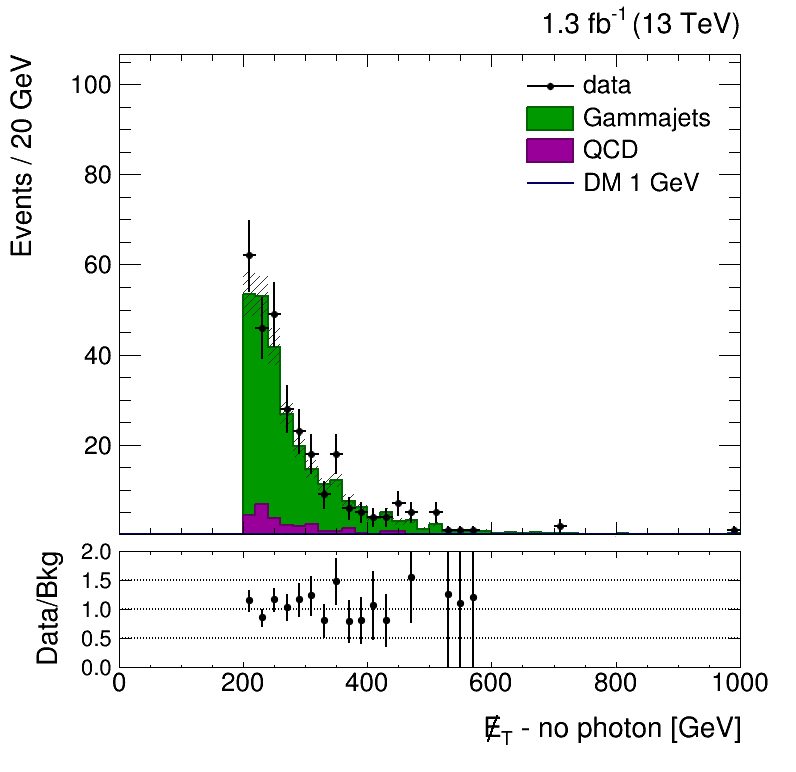
\includegraphics[width=0.48\textwidth]{figures/hPFMETnopholinear_CRzjets.png}
  \caption{The $\met$ distribution in the $\Zjets$ control region with photons for the hadronic channel.}
  \label{fig:incl_hadronic_pho_fmet}
\end{figure}

\subsubsection{Control region for QCD}
\label{subsubsec:bkg_hadronic_qcd}

To obtain a control region enriched in QCD, consider events with no $\Bot$-tagged jets and $\min_{i=1,\ldots,6}\Delta\phi\left(j_i,\,\met\right)<1$. Typically, MC samples for QCD are very statistically limited so the purpose of the control region is to verify that QCD is negligible by looking at the level of data/MC agreement as $\min_{i=1,\ldots,6}\Delta\phi\left(j_i,\,\met\right)$ approaches $1$. If the agreement is good, then it can be concluded that the QCD contribution is negligible. The $\Delta\phi$ distribution in this region is shown in Fig.~\ref{fig:incl_hadronic_qcd_dphijetmet}.

\begin{figure}[htbp]
  \centering
  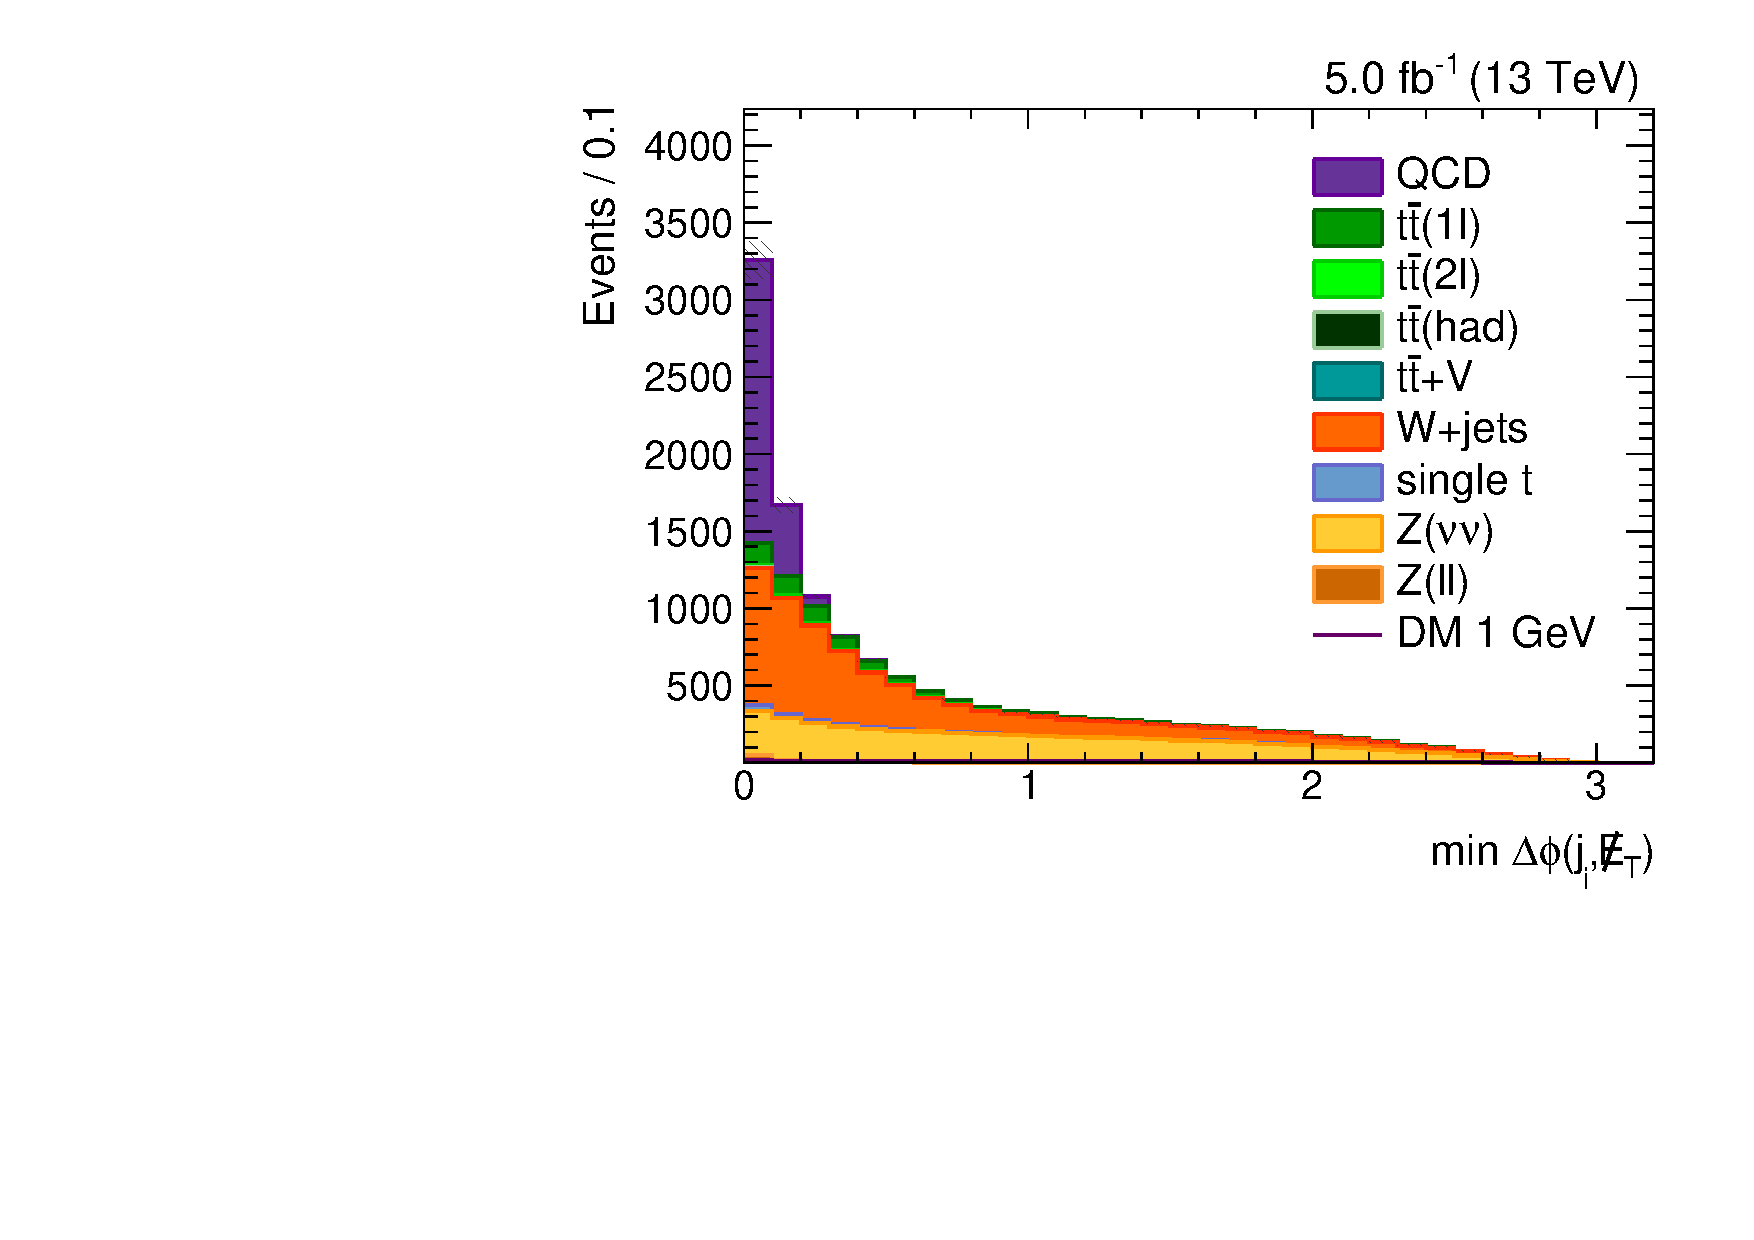
\includegraphics[width=0.48\textwidth]{figures/hadronic-incl-qcd-dphijetmet.pdf}
  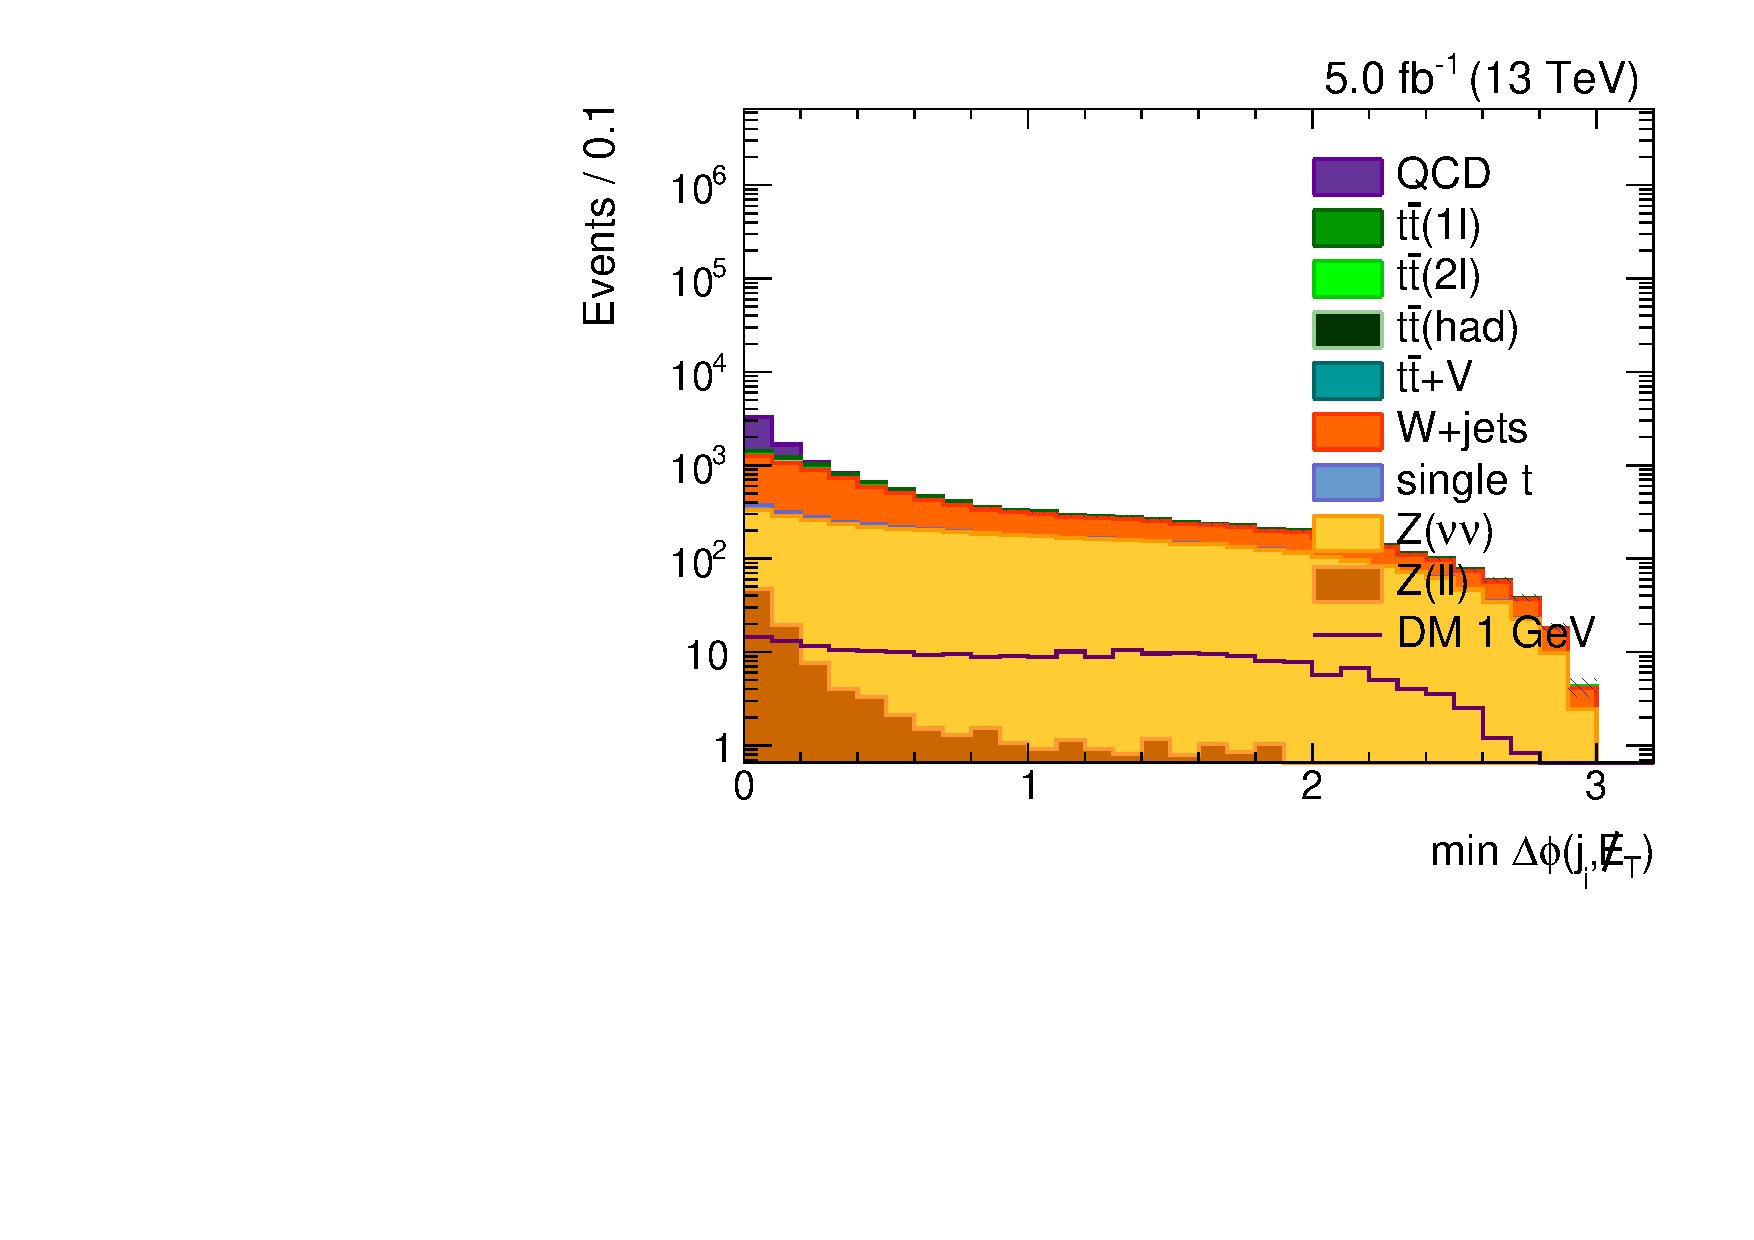
\includegraphics[width=0.48\textwidth]{figures/hadronic-incl-qcd-dphijetmetlog.pdf}
  \caption{The $\min_{i=1,\ldots,6}\Delta\phi\left(j_i,\,\met\right)$ distribution in the QCD control region for the hadronic channel.}
  \label{fig:incl_hadronic_qcd_dphijetmet}
\end{figure}
